\chapter{Next Steps}

%In this chapter I will describe the best possible support elements in detail and will elaborate on their weaknesses and strengths and what further tests should be done to confirm my findings.
%As well as possible alterations to the rig in order to conduct further tests.

Drop tests can only judge the mechanical properties of support components. When designing a support system other factors are also at play. The usability of a support component is not just dependent on its mechanical properties such as energy absorption capacity or displacement capacity. Economical factors are also at play.
The potential to mechanise or automate the installation is an important factor when considering the usability of a support element. Especially in countries with high labor cost, such as Sweden.
The longevity of a component should match the lifespan of the excavation it's supporting. Excessive moisture and acid mine drainage can destroy support elements prematurely. \autocite[2]{player04} \autocite[8]{Simser07} Corrosion plays a part in bolt failures during rock falls. \autocite[8]{villa13} When following up with the research done in this thesis such factors will have to be taken into account. 

The testing method has not been exhaustively optimised. The drop test rig in its current form still has a lot of untapped potential. For example the sensor array could still be improved.
%There are a lot of possible chances to enhance the rig. In its current state only a fraction of its potential is realized.


\section{High Speed Camera}
%A better highspeed camera than the Casio Exilim Pro Ex-F1 might 
The high speed camera footage allows for visual inspection of the data and provides a secondary way to measure displacement. %As of yet no tests have been run using the Phantom Miro LC110 therefore no comment can be made on how it improves the test results. 
So far the high speed camera is very failure prone. By integrating it in the data logger some handling mistakes could be avoided. Then the measurements could also be synchronized. 
Measurements could also be synchronized without integration. For example by turning on an LED at known point in time.

The high speed camera needs high ambient light for best results. Sourcing this light can be difficult. LEDs are known to flicker but at the frame rates that were used so far (up to 5000 fps) this did not impact the quality of the measurements.
Finding enough power outlets is another problem. The test rig only has 5 electrical outlets and when deploying a high speed camera with corresponding laptop needed to control it and several light sources this amount of outlets is insufficient. The resulting amount of drawn power triggered the breakers several times during testing.

\section{Laser Sensor}

%The laser sensor works by measuring the change in the intensity of the laser beam. When the object that the laser is pointed at moves towards the laser the light intensity increases. When the ambient light is bright enough the sensor does not register this change anymore. Therefore low ambient light is favorable when using a laser sensor. Using both high speed camera and laser sensor at the same time would require a compromise in both of their effectiveness. Or a conscious choice for one over the other. The laser sensor is more precise and allows drawing of load displacement curves but it is much more failure prone than the high speed camera. The high speed camera creates visually pleasing videos that can be used for qualitative analysis and representative purposes.

The laser sensor is sensitive to dust or debris falling through the laser beam. Applying the reflective tape to the sample appears to have increased the usability. Still some post processing is required to draw load displacement graphs. Maybe with a different sensor even the need for this could be removed and the data processing could be automated entirely. It would then only require an operator to run the tests and an engineer to look over the graphs. %Especially since the laser sensor and the high speed camera do not work well together. The laser sensor requires low ambient light.

%does not provide reliable data and therefore can not be used in a meaningful way. Therefore our top priority should be to find an alternate way of measuring displacement. Perhaps with an ultrasound sensor, LED sensor or inductive sensors. 

\section{Measuring Velocity}

It would be cautious to measure the impact velocity of the weight somehow in order to confirm the calculated values. Perhaps using two light gates or a line reading camera. Either the variation of impact velocity used in the tests should be minimized or the effects of different velocities would have to be studied. \autocite[25]{Erik15} specifically talks about punching. A failure mode that occurs at high impact velocity, where sample get concentrical cracks in addition to the usual radial ones.

%It would make sense to synchronize the high speed camera with the sensor measurements somehow. Either through integration in the data logger or an LED switching on at a known point in time. It might also be worthwhile considering to trigger the camera together with the other equipment. Currently the highspeed camera has to be triggered manually, which is very failure prone and has already lead to the loss of data from one test.%Also a different camera would probably have to be triggered remotely just before the impact, because of limited data storage capacity.

\section{Load Cells}

Currently the load cells are located at the corners of the concrete slab which imposed the static load. There is no real world equivalent for this force. As such it would make more sense to instead have load cells at the bolt points, to capture the stresses which would be inflicted on the bolts in the given scenario. Such load cells exist and are called force rings.

\section{Drop Weight}

To ascertain the influence the weight pf the drop weight has on the outcome of a test all drop weight should be tested. One option would be to try every drop weight at the same energy level and then at the same impact speed. 
Like this the influence of the impact speed could be determined.

\section{Direct Sensors}

More direct sensors would reveal more about how the sample behaves under load. But these sensors can influence the result positively or negatively. In case of the additional accelerometers the influence was obviously negative. The reasons would need more investigation. The use of the current system is discouraged. The accelerometers could alternatively be screwed directly into the sample.

\section{Testing Surface Support}
\label{sec:mesh}

In the current setup there is very little space for displacement. Too little for the testing of mesh, especially chain-link or textile mesh, which are known for their capacity to deform heavily. Lifting the impact table should be considered in order to increase the testability of different mesh types. Additionally to mesh, different types of straps or lacing should be tested as well. The only type of strap currently in use at Kiirunavaara mine is called %Fjällband, which is currently only used in a very specific use case, will also be tested.
 Fjällband. It is currently only applied laterally between crosscuts in order to  hold the pillars together. %This usecase is generally refered to as a "bull nose". 
 %Fjällband might have a lot of potential or could be entirely cosmetic but there is simply no possible way to know it is tested. 
 There is very little to no documentation on Fjällband so additional tests such as pull strength or shear strength tests, are advisable. Also it might give interesting results to test Fjällband not just singly but also crossed. It has never been applied in such a fashion in the mine but there might be a positive effect.

%There are plans to test lacing. But only one type of steel rope. 
Lacing is a very undefined concept. There are no defined diameters or rope types. Therefore it would make sense to test a lot of different ropes. Lacing is usually steel rope. Synthetic rope could prove to be and interesting alternative.
%Maybe synthetic rope could be an interesting alternative.

%In order to be able to test lacing as well a contraption to attach lacing cables to the frame will be build. 
\section{Sample Preparation and Post Processing}

%Sample preparation is a very important factor. %A quick fix might seem attractive but will carry a host of difficulties. It might make more sense to make a more complicated modification now, that requires less work in sample production later. 

There are four key attributes a test can have.
It can be realistic or abstract, lean or extensive.

Realistic means that the testing conditions are as close to the \textit{in - situ} conditions as possible. %This means that the test has low repeatability, needs more preparation than a more abstract test and is more cost and time intensive.

Abstract tests take the \textit{in - situ} conditions and try to simplify them as far as possible and make the result test procedure more repeatable and cheaper. 

Extensive tests try to gather as much data as possible and decide in post-processing what is useless and what is useful. This kind of tests takes a lot of time in preparatory work and in post processing. If there is not much experience with the testing method extensive tests are a good first step. The results can be surprising and entirely unexpected.

Lean tests are reduced to the bare minimum of preparatory work, sensors array and post-processing. This makes them cheap and fast to run. But a lot of decisions have to made beforehand. It is much harder to have unexpected results or discover new things with a lean test. Lean tests work best if there is already experience with the subject matter and the goal of the experiments is very well defined.

Drop tests are more abstract than blast tests. Repeatability, low running cost and high test frequency are their strong suit. The round panel tests are very abstract, the square tests try to be more realistic. The current sensor array is quite extensive and includes a few redundancies. It could be probably be shrunk without decreasing the quality of the analysis. 

%The question poses itself how in-depth the future analysis of results has to be. 

In this thesis it has been proven that the impact velocity and the impact energy can be estimated with good precision using the mass of the drop weight and the drop height. 

For each parameter that is being measured or could be measured the following questions should be asked.

In the best case scenario, what can we learn from measuring this parameter? Is it important to know the exact value? Is an estimation good enough? Does it correlate or depend on other parameters? How would the analysis of test results be influenced if it was neither measured nor estimated?

If the knowledge of a parameter in the best possible scenario is not interesting or relevant it does not make sense to measure it at all. 
Exact values are more expensive than estimations. The price of sensors increases with their precision. Therefore more exact values are more expensive. Precise values require additional time in both preparation and post processing when compared to estimations. If a parameter correlates with or is dependant on other parameters or if it does not influence the analysis of the test results it might redundant and could perhaps be removed. If it has little influence on the analysis of the test results it does not need to be measured redundantly. If a value has a strong influence on the analysis of the test results it should be to measured redundantly. 

%The additional accelerometers require a lot of preparatory work. The metal plates to which they are attached need to be manufactured and can not be reused. The metal plates need to be glued on at least a day in advance so that the glue can harden sufficiently. The data gathered from the additional accelerometers, the built-in sensors and the high speed camera has to be synchronised in post processing. The data from the laser sensor needs to be cleaned up to be usable. All of which requires valuable time. 

%This thesis tries to provide the reader with the knowledge to necessary to decide which of these sensors are redundant and which are vital. %This poses the question: is all this data really necessary?

%The strong point of impact tests is their repeatability, their low running cost and the high volumes of tests that can be run in a short time frame. All of which would suffer greatly from a high overhead as would be imposed by elaborate preparatory work. The additional accelerometers already require additional work. The metal plates to which they are attached need to be manufactured and can according to our current knowledge not be reused. The metal plates need to be glued on at least a day in advance so that the glue can harden sufficiently. The data gathered from these sensors and the high speed camera has to be synchronised in post-processing. The data from the laser sensor needs to be cleaned up to be usable. All of which requires valuable time. This poses the question: is all this data really necessary? %Is it even possible to turn it into information without being overwhelmed? 
Maybe it would be easier to just find a quick way of measuring post peak capabilities of the system and then present those together with the energy level of the impact and ignoring all the other values. It´s simply a question if running a few very well monitored tests or a lot of simpler tests with a leaner sensor array is preferable. The round sample tests are easier to conduct than the large sample tests and round samples can be produced quicker and are cheaper. Maybe a two step system would be best. First round sample tests could be run with little instrumentation and used for pre-selection. The remaining sample types could then tested in a larger scale with more instrumentation and more careful analysis. Before having such considerations about the testing paradigm it might be worth considering what could be changed about the samples.

\begin{comment}
%Outer confinement changes the behaviour of mesh significantly. Therefore it might be interesting to be able to confine ductile materials such as mesh with varying stiffness or not at all edges.
\begin{figure}
    \centering
    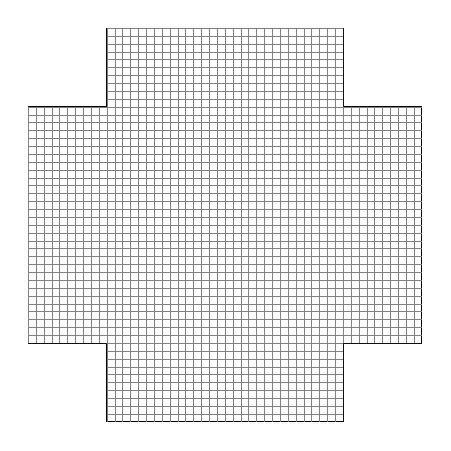
\begin{tikzpicture}
%top view clover leaf mesh

%draw the clip path
\path[clip, draw] (1,0) -- (1,1) -- 
(0,1) -- (0,4) -- (1,4) -- 
(1,5) -- (4,5) -- (4,4) -- (5,4) 
-- (5,1) -- (4,1) -- (4,0) --cycle ;

%draw the mesh
\draw [help lines, step = .1cm] (0,0) grid (6,6);



\end{tikzpicture}
    \caption{Necessary shape of mesh to create the right boundary conditions} 
    \label{fig:meshBound}
\end{figure}
\end{comment}
\begin{comment}
\begin{figure}
    \centering
    
    \subcaptionbox{Sideview of a possible way to produce stiff boundary conditions \label{fig:sideBound}}{
    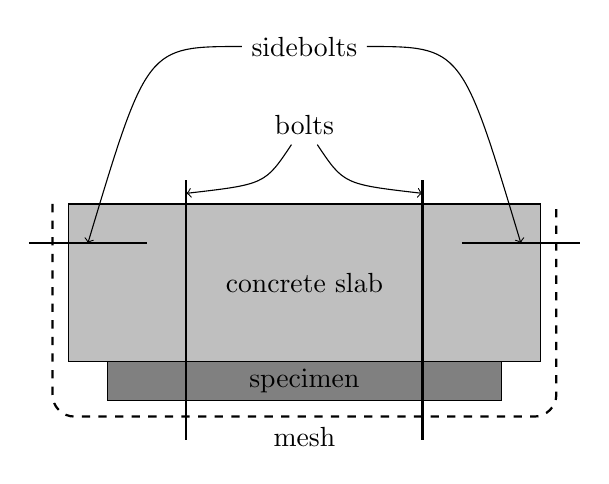
\begin{tikzpicture}
%TOP VIEW OF MESH BOUNDARY

%concrete slab
\filldraw[fill=lightgray] (0,0) rectangle (6,2)
node[pos=.5] {concrete slab};

%sample
\filldraw[fill=gray] (0.5,0) rectangle (5.5,-0.5)
node[pos=.5] {specimen};

%mesh
\draw[thick,rounded corners = 8pt, dashed] (-0.2,2) -- (-0.2,-0.7) -- (6.2,-0.7) node [midway, below] {mesh} -- (6.2,2);

% bolts
\draw[thick]
(1.5,2.3) -- (1.5,-1)
coordinate [pos=0.05] (bolt1)
(4.5,2.3) -- (4.5,-1)
coordinate [pos=0.05] (bolt2);

%sidebolts
\draw[thick] (-0.5,1.5) -- (1,1.5)
coordinate [pos = 0.5] (sbolt1)
(5,1.5) -- (6.5,1.5)
coordinate [pos = 0.5] (sbolt2);

%BOLTS
\draw (3,3) node (bolts) {bolts}
[->] (bolts) .. controls ++ (-0.5,-0.75) .. (bolt1);
\draw [->] (bolts) .. controls ++ (0.5,-0.75) .. (bolt2);

%SIDEBOLTS
\draw (3,4) node (sbolts) {sidebolts}
[->] (sbolts) .. controls ++ (-2,0) .. (sbolt1);
\draw [->] (sbolts) .. controls ++ (2,0) .. (sbolt2);



%what else do I want in here??
%the side bolts
%maybe a sketch of the loom
%pretty graphics anyway

\end{tikzpicture}
    }
    \subcaptionbox{Necessary shape of mesh for this set up \label{fig:meshBound}}
    {
    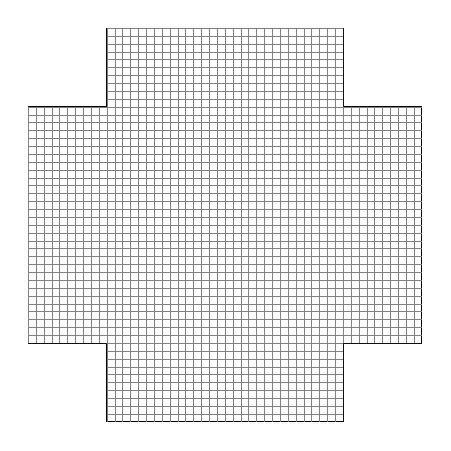
\begin{tikzpicture}
%top view clover leaf mesh

%draw the clip path
\path[clip, draw] (1,0) -- (1,1) -- 
(0,1) -- (0,4) -- (1,4) -- 
(1,5) -- (4,5) -- (4,4) -- (5,4) 
-- (5,1) -- (4,1) -- (4,0) --cycle ;

%draw the mesh
\draw [help lines, step = .1cm] (0,0) grid (6,6);



\end{tikzpicture}
    }

\caption{One possibility of creating stiff boundary conditions}
\label{fig:stiffBound}
\end{figure}

Especially chain-link mesh´s strength lies in its ability to transfer load across a large area which is very hard to replicate. There are a few ideas floating around, some of which are more complicated to manufacture than others. In \autoref{fig:stiffBound} one idea is displayed. In \autoref{fig:sideBound} a side view of the idea is given. The basic principle would be to pull up and attach the mesh to the sides of a concrete slab. Possible ways of attachment would be addition bolts for example. The drawbacks of this method lie in the very difficult sample preparation, firstly the corners would need to be cut from each sample to give it a clover leaf shape as displayed in \autoref{fig:meshBound}.% additionally the "leaves" would have to be bend at a 90 degree angle without breaking any of the wires or welds. Another idea was to built a sort of comb / loom which would not require any bending of the mesh, but this topic will require further discussion in order to solve. 
\end{comment}




%Especially because of the boundary conditions \textit{in - situ}, the the welded mesh panels currently in use have a size of 2,3 on 2,2 m and a bolt spacing of 1 bolts per meter. See \autoref{fig:insituMesh}. Which means that a 1 x 1 m square of mesh has two open boundaries and two flexible boundaries (illustrated in \autoref{fig:insituMesh} with red dashed lines). At least welded mesh panels should be tested in such a way, that these boundary conditions are properly reflected. Which means that two ends of the mesh should be free and two should be constrained somehow. 
 
\section{Concrete and Shotcrete}

According to the current plan, all specimens made from concrete will be cast instead of sprayed. Therefore they are likely to exhibit better properties than could be expected in the field. Spraying the samples would be additional work but the test results would gain credibility. At least  a few tests should be run with shotcrete in order to give some guidance on the reduction in strength that could be expected if such a specimen production regime had been implemented.

\section{Adhesion Between Sample and Concrete Slab}

All currently planned samples will use the adhesion between sample and concrete block. It might be interesting to see how large this adhesion is and therefore a few sample without it should be tested.

The concrete slab is costs a lot of material, makes the samples much harder to handle and increases the sample production time. The value it adds to the experiments has to be worth this cost. Until this worth is not proven, using the concrete slabs is questionable.

\section{Thickness of the Concrete}

It is hard to judge the effect the thickness of the concrete has on its energy adsorptions capabilities. The force measured by the load cells and the acceleration of the drop weight appear to be independent of the thickness of the sample. Just the deformations (which were problematic to measure in the past) and the crack patterns appear to be affected by the thickness. Maybe the accelerometers attached directly to the sample would be affected as well, but as there were no tests conducted with additional accelerometers and a thickness other than 75 mm it is impossible to say.
%are no more tests planned with a thickness other than 75 mm it will be impossible to find out.

%It might be interesting to look into TSL as an alternative to shotcrete. 

\section{Degree of Destruction}

To quantify to the degree of destruction of the samples after a test the displacement and the size of the resulting cracks was measured. These did not correlate with the energy level at all. It appears that the formation of cracks is much more dependant on the sample composition than on the impact energy. 
Maybe a different way of measuring the destruction of a sample should be considered. The very simple division into the two categories "broken" and "cracked" is not quantitative. 
One way could be conducting a quasi-static test after a dynamic test on the same sample. This way  the post-peak capabilities of the sample could be determined. 

\section{Quasi-Static Test Rig}

In order to understand the properties of the tested samples better it would be interesting to know their static load capabilities. Therefore adding a quasi static test facility to the existing rig might be worthwhile. The most important factor when considering this is the magnitude of the required precision. A basic idea, which is to say a margin of error of a few percent or more, should be sufficient. It seems better to have some idea about this than none whatsoever. If it turns out that the static capabilities are more interesting that previously thought the rig can always be upgraded further. 

As the formation of cracks is quite random, the quasi static capabilities might be too. Therefore knowledge of the static capabilities might add little value to the analysis of the test results. %it does not make sense to waste too many resources on it.

%It might be interesting to not just test the static capabilities alone but to test the static capabilities that remain after an impact test. This would give an idea about the post peak capabilities of the tested surface support.

%\section{Post peak capabilities}

%With the current rig the post peak capabilities are hard to assess. Some thought should be put into how this could be done in a qualitative way. 

\section{Bolt Test Rig}

The current rig cannot tests bolts. It might be interesting to tests bolts both dynamically and statically. Something to consider would be to not just test the tensile strength but to also consider ways to test the shear strength. Often the shear strength of bolts is not considered when designing a support system but it often leads to failure during rockbursts. \autocite[17]{guler01} When the rig has the ability to test bolts it's not a very large step to testing bolts and surface support together as a support system.

\section{Support System}

 It might be very interesting in the future to inspect the interplay of different surface support concepts with different bolts. To achieve this, the threaded bars that serve as bolts would need to be replaced with real bolts. The samples would need to be suspended by the bolts instead of resting on the load cells and instead forces would need to be measured using for example force ring located between bolt plate and concrete.
 
%This list does not claim to be exhaustive but merely a collection of suggestions. With all these possible enhancement and modifications in mind it is crucial to prioritize and focus on what is really important.





